\documentclass[11pt]{article}

\usepackage{fullpage}
\parindent=0in

\def\changemargin#1#2{\list{}{\rightmargin#2\leftmargin#1}\item[]}
\let\endchangemargin=\endlist 

%------------------------------------------------------------------
% PROBLEM, PART, AND POINT COUNTING...

% Create the problem number counter.  Initialize to zero.
\newcounter{problemnum}

% Specify that problems should be labeled with arabic numerals.
\renewcommand{\theproblemnum}{\arabic{problemnum}}


% Create the part-within-a-problem counter, "within" the problem counter.
% This counter resets to zero automatically every time the PROBLEMNUM counter
% is incremented.
\newcounter{partnum}[problemnum]

% Specify that parts should be labeled with lowercase letters.
\renewcommand{\thepartnum}{\arabic{partnum}}

% Make a counter to keep track of total points assigned to problems...
\newcounter{totalpoints}

% Make counters to keep track of points for parts...
\newcounter{curprobpts}		% Points assigned for the problem as a whole.
\newcounter{totalparts}		% Total points assigned to the various parts.

% Make a counter to keep track of the number of points on each page...
\newcounter{pagepoints}
% This counter is reset each time a page is printed.

% This "program" keeps track of how many points appear on each page, so that
% the total can be printed on the page itself.  Points are added to the total
% for a page when the PART (not the problem) they are assigned to is specified.
% When a problem without parts appears, the PAGEPOINTS are incremented directly
% from the problem as a whole (CURPROBPTS).


%---------------------------------------------------------------------------


% The \problem environment first checks the information about the previous
% problem.  If no parts appeared (or if they were all assigned zero points,
% then it increments TOTALPOINTS directly from CURPROBPTS, the points assigned
% to the last problem as a whole.  If the last problem did contain parts, it
% checks to make sure that their point values total up to the correct sum.
% It then puts the problem number on the page, along with the points assigned
% to it.

\newenvironment{problem}[1]{
% STATEMENTS TO BE EXECUTED WHEN A NEW PROBLEM IS BEGUN:
%
% Increment the problem number counter, and set the current \ref value to that
% number.
\refstepcounter{problemnum}
%
% Add some vspace to separate from the last problem.
\vspace{0.15in} \par
%
\setcounter{curprobpts}{#1} \setcounter{totalparts}{0}	% Reset counters.
%
% Now put in the "announcement" on the page.
\noindent{\Large \bf Question \theproblemnum. \normalsize ({\it \arabic{curprobpts} point\null\ifnum \value{curprobpts} = 1\else s\fi}\/)}
}{
% STATEMENTS TO BE EXECUTED WHEN AN OLD PROBLEM IS ENDED:
%
% If no parts to problem, then increment TOTALPOINTS and PAGEPOINTS for the
% entire problem at once.
\ifnum \value{totalparts} = 0
	\addtocounter{totalpoints}{\value{curprobpts}}	% Add pts to total.
	\addtocounter{pagepoints}{\value{curprobpts}}	% Add pts to page total.
%
% If there were parts for the problem, then check to make sure they total up
% to the same number of points that the problem is worth. Issue a warning
% if not.
\else \ifnum \value{totalparts} = \value{curprobpts}
	\else \typeout{}
	\typeout{!!!!!!!   POINT ACCOUNTING ERROR   !!!!!!!!}
	\typeout{PROBLEM [\theproblemnum] WAS ALLOCATED \arabic{curprobpts} POINTS,}
	\typeout{BUT CONTAINS PARTS TOTALLING \arabic{totalparts} POINTS!}
	\typeout{}
	\fi
\fi
}


%---------------------------------------------------------------------------


% The \newpart command increments the part counter and displays an appropriate
% lowercase letter to mark the part.  It adds points to the point counter
% immediately.  If 0 points are specified, no point announcement is made.
% Otherwise, the announcement is in scriptsize italics.

\newcommand{\newpart}[2]{
\refstepcounter{partnum}	% Set the current \ref value to the part number.
\begin{changemargin}{0in}{0in}
  \noindent\textbf{\theproblemnum.\thepartnum}~(\textit{#1 points}): 
  \textit{ #2}
\end{changemargin}
\addtocounter{totalparts}{#1}	% Add points to totalparts for this problem.
\addtocounter{pagepoints}{#1}	% Add points to total for this page.
\addtocounter{totalpoints}{#1}	% Add points to total for entire test.
}

\newcommand{\answerpart}[1]{
\begin{changemargin}{0.25in}{0in}
\noindent \textbf{Answer:} {#1}
\end{changemargin}	
}

\newcommand{\answer}[1]{
\textbf{Answer:} {#1}
}



%---------------------------------------------------------------------------



% Just in case you want to skip some numbers in your test...

\newcommand{\skipproblem}[1]{\addtocounter{problemnum}{#1}}



%---------------------------------------------------------------------------


% The \showpoints command simply gives a count of the total points read in up to
% the location at which the command is placed.  Typically, one places one
% \showpoints command at the end of the latex file, just prior to the
% \end{document} command.  It can appear elsewhere, however.

\newcommand{\showpoints}
{
\typeout{}
\typeout{====> A TOTAL OF \arabic{totalpoints} POINTS WERE READ.}
\typeout{}
}


%---------------------------------------------------------------------------



\usepackage{graphicx}
\usepackage[english]{babel}
\usepackage[latin1]{inputenc}
\usepackage{times}
\usepackage[T1]{fontenc}
\usepackage{amsmath}
\usepackage{amssymb}
\usepackage{booktabs}

\newcommand{\argmax}{\mathop{\arg\max}}
\newcommand{\deriv}[1]{\frac{\partial}{\partial {#1}} }
\newcommand{\dsep}{\mbox{dsep}}
\newcommand{\Pa}{\mathop{Pa}}
\newcommand{\ND}{\mbox{ND}}
\newcommand{\De}{\mbox{De}}
\newcommand{\Ch}{\mbox{Ch}}
\newcommand{\graphG}{{\mathcal{G}}}
\newcommand{\graphH}{{\mathcal{H}}}
\newcommand{\setA}{\mathcal{A}}
\newcommand{\setB}{\mathcal{B}}
\newcommand{\setS}{\mathcal{S}}
\newcommand{\setV}{\mathcal{V}}
\DeclareMathOperator*{\union}{\bigcup}
\DeclareMathOperator*{\intersection}{\bigcap}
\DeclareMathOperator*{\Val}{Val}
\newcommand{\mbf}[1]{{\mathbf{#1}}}
\newcommand{\eq}{\!=\!}
\usepackage[usenames,dvipsnames]{color}
\newcommand{\bto}[1]{\textcolor{Bittersweet}{[#1 -BTO]}}

\newcommand{\update}[1]{\textcolor{blue}{[#1]}}

\newcommand{\HR}{\mathrm{HR}}
\newcommand{\A}{\mathrm{A}}
\newcommand{\HD}{\mathrm{HD}}
\newcommand{\CH}{\mathrm{CH}}
\newcommand{\BP}{\mathrm{BP}}
\usepackage{hyperref}

\begin{document}

{\centering
  \rule{6.3in}{2pt}
  \vspace{1em}
  {\Large
    CS688: Graphical Models - Spring 2020 \\
    Assignment 1\\
  }
  \vspace{1em}
  Assigned: Tuesday, Feb 11 Due: Friday, Feb 21 at 5:00pm \\
  \vspace{0.1em}
  \rule{6.3in}{1.5pt}
}
\vspace{1pc}


\textbf{General Instructions:} Please upload {\em\bf two items} to \textit{Gradescope} (\url{https://www.gradescope.com/courses/86501}): (1) a report with your answers (\textit{.pdf}), and (2) a zip file with your code (\textit{.zip}).\\
Submit a report with the answers to each question. You are encouraged to typeset your solutions. To help you get started, the full \LaTeX source of the assignment is included with the assignment materials. For your assignment to be considered ``on time'', you must upload both (1) and (2) to \textit{Gradescope} by the due date. Make sure the code is sufficiently well documented that it's easy to tell what it's doing. You may use any programming language you like. For this assignment, you may not use existing code libraries for Bayesian network modeling, learning or inference. If you think you've found a bug with the data or an error in any of the assignment materials, please post a question to the Piazza discussion forum. Make sure to list in your report any outside references you consulted (books, articles, web pages, etc.) and any students you collaborated with.\\
When you submit reports through \textit{Gradescope}, you are supposed to mark what part of the .pdf corresponds to each question. Please note that you will lose credit on this assignment if you fail to do this. \\

\textbf{Academic Honesty Statement:} You are encouraged to {\it discuss} with other students to understand the material, but not to share solutions.
Copying solutions from external sources (books, web pages, etc.) or other students is considered cheating, and so is sharing your solutions. At no point should another student see your solutions. \\

\textbf{Introduction:} In this assignment, you will experiment with different aspects of modeling, learning, and applying a Bayesian network to answer probability queries. This assignment focuses on the heart disease diagnosis domain and uses part of a real clinical data set. \\

\textbf{Data Set:} The data set consists of 9 variables as described below. The number of each variable corresponds to its column number in the data set files. There are five sets of training and test data files in standard comma-separated-value (CSV) format. The files are named \textit{data-train-i.txt} and \textit{data-test-i.txt} for $i$ from $1$ to $5$.\\

\begin{center}
\scalebox{.87}{
\begin{tabular}{llll}\toprule
Number & Name & Description & Values\\ \midrule
1 & A   &  Age          & 1:$<45$, 2: $45-55$, 3:$\geq 55$\\ 
2 & G   &  Gender                  & 1:Female, 2:Male;\\ 
3 & CP  &  Chest Pain & 1:Typical, 2:Atypical, 3:Non-Anginal, 4:None\\ 
4 & BP  &  Blood Pressure          & 1:Low, 2:High\\ 
5 & CH  &  Cholesterol             & 1:Low, 2:High\\ 
6 & ECG &  Electrocardiograph      & 1:Normal, 2:Abnormal\\ 
7 & HR  &  Exercise Heart Rate     & 1:Low, 2:High\\ 
8 & EIA &  Exercise Induced Angina & 1:No, 2:Yes\\ 
9 & HD  & Heart Disease            & 1:No, 2:Yes\\ \bottomrule
\end{tabular}}
\end{center}

\textbf{Model: } We will consider applying a Bayesian network with the following structure to the data set.\\

\begin{center}
    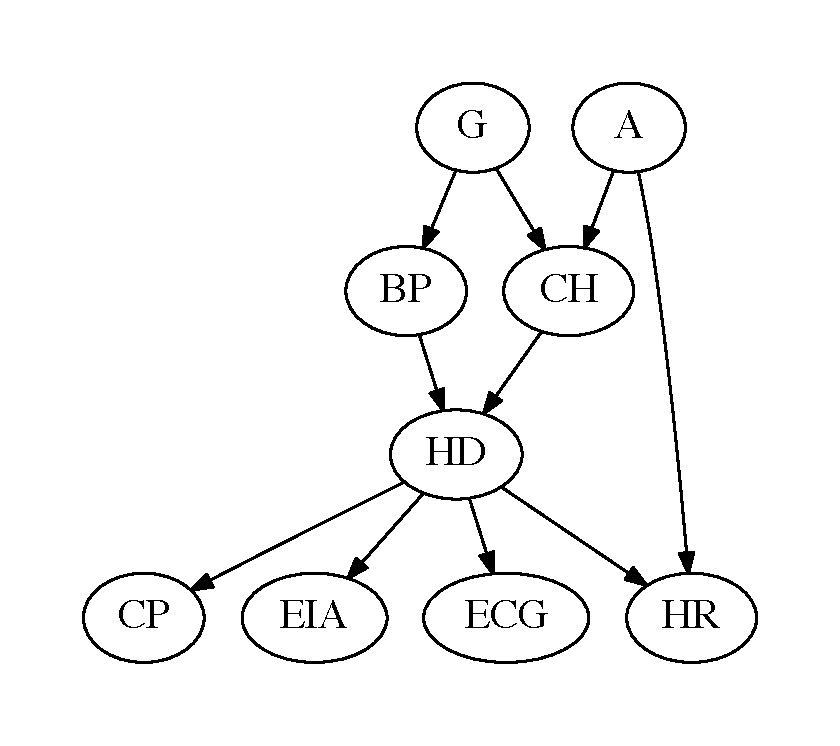
\includegraphics[scale=0.5,trim=10mm 10mm 10mm 10mm,clip]{bn.pdf}
\end{center}

\begin{problem}{10} \textbf{Factorization:} Write down the factorization of the Bayesian network joint distribution implied by the structure shown above. 
\end{problem}


\begin{problem}{10} \textbf{Likelihood Function:} Write down the log likelihood of the Bayesian network model as a function of the parameters $\theta$ given $N$ data cases. For this problem use the notation for the parameters of conditional probability tables discussed in class e.g.
  \[ p_{\theta}(HD=hd \mid CH=ch,BP=bp)=\theta^{\HD|\CH,\BP}_{hd|ch,bp}. \]
\end{problem}

\begin{problem}{15} \textbf{Maximum Likelihood Estimates:} Again using the above notation for the parameters, derive the maximum likelihood estimate for the parameter $\theta^{\HR|\A,\HD}_{L|1,Y}$ starting from the log likelihood function.  Be sure to account for the sum-to-one constraint $\sum\limits_{hr\in\{L,H\}} \theta^{\HR|\A,\HD}_{hr|1,Y}=1$.  Show your work.
\end{problem}

\begin{problem}{15} \textbf{Learning:} Implement the maximum likelihood parameter estimates for all CPTs in the model. For this question, run your code on the data in the \textit{first training data set only} to compute the maximum likelihood parameter estimates for each CPT in the model. Report the maximum likelihood values you computed for each of the following CPTs:\\
	
\textbf{(a)} $p_{\theta}(A)$\\
\textbf{(b)} $p_{\theta}(BP|G)$\\
\textbf{(c)} $p_{\theta}(HD|BP,CH)$\\
\textbf{(d)} $p_{\theta}(HR|A,HD)$\\

You may report the values of the above CPTs using the provided template \textit{params.pdf}. Or, you may also write code to output the CPTs, which is strongly recommended. However, make sure to list the CPTs in your report in the order they appear in the supplied template. Also make sure to list the configurations within each CPT in the same order that they appear in the template. This is to facilitate grading. 
\end{problem}

\begin{problem}{15} \textbf{Probability Queries:}
For each of the two queries below, first show how the query can be expressed in terms of the factorized joint distribution for the Bayesian network. Simplify the expressions wherever possible using the conditional independence properties of the network structure. Finally, use the parameters obtained in the previous question (first training set file only) to compute the distribution over the query variables. Display the result using a table or a bar chart. Note that there is an unobserved variable in the second query.\\

\textbf{(a)} {\footnotesize $p(CH|A=2,G=M,CP=\text{None},BP=L,ECG=\text{Normal},HR=L,EIA=\text{No},HD=\text{No})$}\\
\textbf{(b)} {\footnotesize $p(BP|A=2,CP=\text{Typical},CH=H,ECG=\text{Normal},HR=H,EIA=\text{Yes},HD=\text{No})$}

\end{problem}

\begin{problem}{20} \textbf{Classification:}
In this question, we will assess the ability of the model to correctly predict the occurrence of heart disease given the values of all of the other variables in the network. Perform the following steps:\\

\textbf{(a)} Train the network on each of the five training data files, obtaining five sets of parameters. There is nothing to report for this step. \\

\textbf{(b)} Write down the probability distribution over the heart disease variable (HD) given the remaining variables. Simplify the result using the conditional independence properties of the network. \\

\textbf{(c)} We will follow a standard five-fold-cross validation protocol to assess the performance of the model. For each test file $i$ and each test data case $n$, compute the most likely value of the heart disease variable $\hat{hd}_{ni}$ using the parameters learned with training file $i$. For each test file $i$, compute the prediction accuracy $A_i$ as the number of cases correctly predicted divided by the total number of cases. Lastly, compute the mean prediction accuracy over the five test files (the average of $A_1$ to $A_5$) and the standard deviation of the prediction accuracy over the five test files (the standard deviation of $A_1$ to $A_5$). Report the mean and the standard deviation of the prediction accuracy.
\end{problem}


\begin{problem}{15} \textbf{Modeling:} Design your own network structure for the heart disease domain. \\

\textbf{(a)} Draw the graphical model for your network. \\

\textbf{(b)} Write down the factorization for your network.\\

\textbf{(c)} Briefly describe some of the choices that went into the design of your network structure.\\

\textbf{(d)} Use your network to repeat the heart disease classification experiment and report the mean and standard deviation of your network. Can you find a network with better accuracy than the given network?
\end{problem}

\showpoints
\end{document} 

